\section{EXPERIENCES AND RESULTS}\label{chap:experiences}

In this section, multiple experiences using both KLEE and Owi tools will be described and analysed. We will start by describing the test environment in \cref{section:test_environment}, and then proceed to summarize the experiments ran in \cref{section:test_samples}. The metrics used to evaluate the tools will be presented in \cref{section:metrics}, and finally a summary of all results and an analysis will be presented in \cref{section:results}.
Each experience will showcase their capabilities and limitations. 

\subsection{Test Environment}\label{section:test_environment}

To increase the results' credibility, all tests were run on the same machine, therefore sharing the same resources. The specifications of such machine consisted in a 12th Gen Intel Core processor (i7-1255U) of 10 cores (and a total of 12 threads) with a max clock speed of 4.70 GHz, and 20 GB (4 + 16) of DDR4 3200 MHz RAM. 

This is the parent system setup with a Windows 11 installation; however, the test environment was created in a WSL environment within this machine which shares 4 cores and 8 GB of RAM available.

For simplicity of testing, all samples were organized by folders and subfolders: the parent folder aggregates by sample and child folders aggregates files by tool, KLEE or Owi.

\subsection{Test Samples}\label{section:test_samples}

To compare the tools we will run them in 9 samples. The samples 1 and 2 were extracted from KLEE's online documentation \cite{klee_tutorial1,klee_tutorial2} and samples 3 through 5 from Owi's GitHub repository \cite{owi_gh}. 
Samples 6 through 9 were recovered from \citeauthor{ADALogicsKLEE} blog \cite{ADALogicsKLEE}. All samples were adapted with necessary changes to ensure compatibility with both tools. They cover, in that order, the following vulnerabilities: 

% \citeauthor{ADALogicsKLEE} \cite{ADALogicsKLEE}
%  presents 4 videos to demonstrate KLEE set of features and in video 3 they discuss vulnerabilities of the types:

\begin{itemize}
    \item Global Buffer Overflow
    \item Stack-based Buffer Overflow
    \item NULL pointer dereference
    \item Use after \lstinline$free$
\end{itemize}

We can look at sample 7 as an example of how KLEE and Owi compare. Stack-based Buffer Overflow vulnerabilities look at scoped and dynamically allocated variables like the one on line 8 of \cref{lst:chap4_sample7_test2}. To run KLEE and Owi on this sample, the sources were instrumented as shown on \Cref{lst:chap4_sample7_klee} and \Cref{lst:chap4_sample7_owi}, respectively.

% Running KLEE results in 6 generated tests, one of which triggered an execution error shown in detail on \Cref{lst:chap4_sample7_klee_test}. This time, the error occurs on \cref{line:4_7_error} of file main (\Cref{lst:chap4_sample7_klee}).
% Owi fails to find the vulnerability on this sample.

% \begin{lstlisting}[
% caption={Sample 7 - KLEE output},
% label={lst:chap4_sample7_klee_output},
% % upquote=true,
% escapechar=@,
% numbers=left,
% breaklines=true,
% postbreak=\mbox{\textcolor{red}{$\hookrightarrow$}\space},
% ]
% KLEE: NOTE: KLEE: ERROR: main.c:26: memory error: out of bound pointer
% now ignoring this error at this location

% KLEE: done: total instructions = 12566
% KLEE: done: completed paths = 5
% KLEE: done: partially completed paths = 1
% KLEE: done: generated tests = 6
% \end{lstlisting}

% \begin{lstlisting}[
% caption={Sample 7 - KLEE test case for the detected error},
% label={lst:chap4_sample7_klee_test},
% % upquote=true,
% escapechar=@,
% numbers=left,
% breaklines=true,
% postbreak=\mbox{\textcolor{red}{$\hookrightarrow$}\space},
% ]
% ktest file : './sample7/klee/klee-last/test000003.ktest'
% args       : ['main.bc']
% num objects: 1
% object 0: name: 'arr'
% object 0: size: 10
% object 0: data: b'BUG!\x00\xff\xff\xff\xff\x00'
% object 0: hex : 0x4255472100ffffffff00
% object 0: text: BUG!......
% \end{lstlisting}

\lstinputlisting[
caption={Sample 7 - test2 function code},
label={lst:chap4_sample7_test2},
language=c,
% upquote=true,
numbers=left,
breaklines=true,
showstringspaces=false,
postbreak=\mbox{\textcolor{red}{$\hookrightarrow$}\space},
]{code-snippets/chap4.sample7/function_test2}

\lstinputlisting[
caption={Sample 7 - KLEE instrumentation},
label={lst:chap4_sample7_klee},
language=c,
% upquote=true,
numbers=left,
breaklines=true,
showstringspaces=false,
postbreak=\mbox{\textcolor{red}{$\hookrightarrow$}\space},
]{code-snippets/chap4.sample7/klee_main}

\lstinputlisting[
caption={Sample 7 - Owi instrumentation},
label={lst:chap4_sample7_owi},
language=c,
% upquote=true,
numbers=left,
breaklines=true,
showstringspaces=false,
postbreak=\mbox{\textcolor{red}{$\hookrightarrow$}\space},
]{code-snippets/chap4.sample7/owi_main}

% \subsection{Sample 8 - NULL pointer dereference}\label{section:sample_8}

% To test NULL pointer dereference bugs, a small string array (`\lstinline$char *global_string[]$' on \cref{line:4_8_global_var}) is initialized and used in function `\lstinline$test3$' where on \cref{line:4_8_error} will trigger an error when the input is favorable.

% After the samples are instrumented, the tools are run and a pattern begins to show where KLEE detects the vulnerability but Owi does not. See \Cref{lst:chap4_sample8_klee,lst:chap4_sample8_owi} for KLEE and Owi instrumented samples, respectively, \Cref{lst:chap4_sample8_klee_output} for KLEE terminal output and \Cref{lst:chap4_sample8_klee_test} for the generated test case.

% \lstinputlisting[
% caption={Sample 8 - Owi instrumentation},
% label={lst:chap4_sample8_owi},
% escapechar=@,
% language=c,
% numbers=left,
% breaklines=true,
% postbreak=\mbox{\textcolor{red}{$\hookrightarrow$}\space},
% ]{code-snippets/chap4.sample8/owi_main}

% \begin{lstlisting}[
% caption={Sample 8 - KLEE output},
% label={lst:chap4_sample8_klee_output},
% % upquote=true,
% escapechar=@,
% numbers=left,
% breaklines=true,
% postbreak=\mbox{\textcolor{red}{$\hookrightarrow$}\space},
% ]
% KLEE: ERROR: main.c:21: memory error: out of bound pointer
% KLEE: NOTE: now ignoring this error at this location

% KLEE: done: total instructions = 12549
% KLEE: done: completed paths = 5
% KLEE: done: partially completed paths = 1
% KLEE: done: generated tests = 6
% \end{lstlisting}

% \begin{lstlisting}[
% caption={Sample 8 - KLEE test case for the detected error},
% label={lst:chap4_sample8_klee_test},
% % upquote=true,
% escapechar=@,
% numbers=left,
% breaklines=true,
% postbreak=\mbox{\textcolor{red}{$\hookrightarrow$}\space},
% ]
% ktest file : './sample8/klee/klee-last/test000003.ktest'
% args       : ['main.bc']
% num objects: 1
% object 0: name: 'arr'
% object 0: size: 10
% object 0: data: b'BUG!\x00\xff\xff\xff\xff\x00'
% object 0: hex : 0x4255472100ffffffff00
% object 0: text: BUG!......
% \end{lstlisting}

% \subsection{Sample 9 - Use after free}\label{section:sample_9}

% Finally, `Use after free' runtime errors can also become very hard to detect by the human eye when code complexity increases; `\lstinline$test4$' function presents a simple case of this vulnerability to showcase KLEE and Owi capabilities. \Cref{lst:chap4_sample9_klee,lst:chap4_sample9_owi} illustrate instrumented sources for each symbolic execution engine.

% KLEE detected the bug on \cref{line:4_9_error}, generated 6 tests, and distinguished the error from the ones on \cref{section:sample_6,section:sample_7,section:sample_8}. KLEE's output (\Cref{lst:chap4_sample9_klee_output}) shows that the memory error is of type `\lstinline$double free$' on \cref{line:4_9_double_free}, and the generated test case (\Cref{lst:chap4_sample9_klee_test}) shows the expected input value.

% \begin{lstlisting}[
% caption={Sample 9 - KLEE output},
% label={lst:chap4_sample9_klee_output},
% % upquote=true,
% escapechar=@,
% numbers=left,
% breaklines=true,
% postbreak=\mbox{\textcolor{red}{$\hookrightarrow$}\space},
% ]
% KLEE: ERROR: main.c:14: memory error: double free@\label{line:4_9_double_free}@
% KLEE: NOTE: now ignoring this error at this location

% KLEE: done: total instructions = 12484
% KLEE: done: completed paths = 5
% KLEE: done: partially completed paths = 1
% KLEE: done: generated tests = 6
% \end{lstlisting}

% \begin{lstlisting}[
% caption={Sample 9 - KLEE test case for the detected error},
% label={lst:chap4_sample9_klee_test},
% % upquote=true,
% escapechar=@,
% numbers=left,
% breaklines=true,
% postbreak=\mbox{\textcolor{red}{$\hookrightarrow$}\space},
% ]
% ktest file : './sample9/klee/klee-last/test000003.ktest'
% args       : ['main.bc']
% num objects: 1
% object 0: name: 'arr'
% object 0: size: 10
% object 0: data: b'BUG!\x00\xff\xff\xff\xff\x00'
% object 0: hex : 0x4255472100ffffffff00
% object 0: text: BUG!......
% \end{lstlisting}

% While KLEE detected the double free as any other code issue, Owi reported the problem as an internal error and its respective stack trace as displayed in \Cref{lst:chap4_sample9_owi_output}. This behaviour suggests the tool does not properly support this issue and might cause the scan to miss other issues because of this internal error.

% \begin{lstlisting}[
% caption={Sample 9 - Owi output},
% label={lst:chap4_sample9_owi_output},
% % upquote=true,
% escapechar=@,
% numbers=left,
% breaklines=true,
% postbreak=\mbox{\textcolor{red}{$\hookrightarrow$}\space},
% ]
% owi: internal error, uncaught exception:
%      Failure("Memory leak double free")
%      Raised at Stdlib__Domain.join in file "domain.ml", line 296, characters 16-24
%      Called from Stdlib__Array.iter in file "array.ml", line 113, characters 31-48
%      Called from Owi__Wq.read_as_seq.(fun) in file "src/data_structures/wq.ml", line 17, characters 4-16
%      Called from Owi__Cmd_sym.cmd.print_and_count_failures in file "src/cmd/cmd_sym.ml", line 99, characters 10-20
%      Called from Owi__Cmd_sym.cmd in file "src/cmd/cmd_sym.ml", line 130, characters 15-49
%      Called from Cmdliner_term.app.(fun) in file "cmdliner_term.ml", line 24, characters 19-24
%      Called from Cmdliner_eval.run_parser in file "cmdliner_eval.ml", line 35, characters 37-44
% \end{lstlisting}

% % \noindent\begin{minipage}{\linewidth}
% \lstinputlisting[
% caption={Sample 9 - Owi instrumentation},
% label={lst:chap4_sample9_owi},
% language=c,
% numbers=left,
% breaklines=true,
% postbreak=\mbox{\textcolor{red}{$\hookrightarrow$}\space},
% ]{code-snippets/chap4.sample9/owi_main}
% % \end{minipage}

\subsection{Metrics}\label{section:metrics}

% Both KLEE and Owi require compiled sources, however Owi can abstract that process for the user if they are testing C source code. To avoid our statistics to include resources spent in source compilation, we will compile our sources for Owi using the same command they do in their abstraction. Please note that the comparisons in \Cref{tab:feature_comparison} - \nameref{tab:feature_comparison} take only symbolic execution features into consideration.

This section discusses \textbf{Accuracy} and \textbf{Performance} metrics such as True Positives (\textbf{TP}), False Positives (\textbf{FP}), True Negatives (\textbf{TN}), False Negatives (\textbf{FN}), and Youden Index (\textbf{J}) also known as Youden's J statistic:

\par\noindent\textbf{\textit{Accuracy Metrics}}
\begin{itemize}
    \item \textbf{TP}: Number of expected vulnerabilities reported.
    \item \textbf{TN}: Number of unexpected vulnerabilities not reported.
    \item \textbf{FP}: Number of unexpected vulnerabilities reported.
    \item \textbf{FN}: Number of expected vulnerabilities not reported.
    \item \textbf{Youden Index}: The accuracy metric used in OWASP Benchmark \cite{owasp_benchmark_scoring} is the following\\ 
    \begin{minipage}{0.6\textwidth}
    \raggedright
    $
      \begin{aligned}
        J & = TPR - FPR = (\frac{TP}{TP+FN}) - (\frac{FP}{TN+FP})
        %   & = \frac{TP*TN-FP*FN}{(TP+FN)(TN+FP)} \\
      \end{aligned}
    $\\
    \vspace{1em}
    \footnotesize{TPR - True Positive Rate}\\
    \footnotesize{FPR - False Positive Rate}\\
    \vspace{1em}
    \end{minipage}
\end{itemize}

When reading the Youden Index, the higher the value, the better the tool is at detecting vulnerabilities. OWASP Benchmark also provides a Youden Index interpretation guide that uses both TPR and FPR values \cite{owasp_benchmark_scoring}.

\par\noindent\textbf{\textit{Performance Metrics}}
\begin{itemize}
    \item \textbf{Paths traced}: Branches of execution created to navigate.
    \item \textbf{CPU (\%)}: The CPU used by the process, in percentage.
    \item \textbf{Memory (KB)}: The `maximum resident set size' (very similar to peak memory) used by the process, in kilobytes.
    \item \textbf{Time (s)}: The execution time of the process, in seconds.
\end{itemize}

Accuracy metrics were extracted by manually inspecting each scan output, and performance metrics such as CPU, memory and time of execution were measured using the GNU \lstinline$time$ program. ``\textbf{Paths traced}'' was also extracted manually similarly to accuracy metrics. There is also the ``\textbf{Success}'' metric that indicates whether the sample was successfully analysed by the test tool, without regard for results.

% \begin{lstlisting}[
% boxpos=ht,
% caption={Extraction of performance metrics},
% label={lst:time_command},
% ]
% # to avoid confusion with bash keyword 'time'
% # use the full path given to you by `which time`

% time -v klee main.bc

% time -v owi sym main.wasm   
% \end{lstlisting}

%%%% ACCURACY

\subsection{Results and Analysis}\label{section:results}

After executing both engines on all test samples and extracting the results from each of them, \Cref{tab:klee_accuracy,tab:owi_accuracy} were created. With these metrics properly formatted, calculating the Youden Index for both tools is easier, higher is better.

It is apparent how KLEE detected much more vulnerabilities than Owi, which plays in its favour, and the calculations on \cref{equ:klee_youden_index,equ:owi_youden_index} reflect this statement, KLEE scores approximately 54\% while Owi stands on 29\% of bug detection accuracy.

If we look at the Youden Index interpretation guide from OWASP Benchmark \cite{owasp_benchmark_scoring}, we can see that KLEE scores highly (87.5\%) in the \textit{y} axis (TPR), while Owi scores poorly (28.5\%). Both tools score low on the \textit{x} axis (FPR), with KLEE at 33.3\% and Owi at 0\%. This means that KLEE is very good at detecting vulnerabilities, but also has a higher rate of false positives, while Owi is not very good at detecting vulnerabilities, but has a low rate of false positives. A larger set of samples would be needed to draw more concrete conclusions.

% KLEE tests table
\begin{table}[tb]
\begin{minipage}{.49\linewidth}
    \centering
    \caption{KLEE accuracy metrics}
    \begin{tabular}{c|c|c|c|c}
        \multicolumn{1}{c|}{\#$^{\mathrm{a}}$} & \multicolumn{1}{c}{TP} & \multicolumn{1}{c}{TN} & \multicolumn{1}{c}{FP} & \multicolumn{1}{c}{FN} \\
        \hline
        \hline
        1 & 0 & 1 & 0 & 0 \\
        2 & 2 & 0 & 0 & 0 \\
        3 & 1 & 0 & 0 & 0 \\
        4 & 0 & 1 & 0 & 0 \\
        5 & 0 & 0 & 1 & 1 \\
        % 5 & YES\rlap{\footnote{KLEE was able to run, but it wasn't able to make use of Frama-C's E-ACSL capabilities}} & 0 & 0 & 1 & 1 \\
        6 & 1 & 0 & 0 & 0 \\
        7 & 1 & 0 & 0 & 0 \\
        8 & 1 & 0 & 0 & 0 \\
        9 & 1 & 0 & 0 & 0 \\
        \hline
        \multicolumn{5}{l}{}\\
        \multicolumn{5}{l}{$^{\mathrm{a}}$\footnotesize{Sample number}} \\
        % \multicolumn{6}{l}{$^{\mathrm{b}}$\footnotesize{The best out of five runs}} \\
    \end{tabular}
    \label{tab:klee_accuracy}
\end{minipage}
% \end{table}
% \begin{table}[htbp]
\begin{minipage}{.49\linewidth}
    \centering
    \caption{Owi accuracy metrics}
    \begin{tabular}{c|c|c|c|c}
        \multicolumn{1}{c|}{\#$^{\mathrm{a}}$} & \multicolumn{1}{c}{TP} & \multicolumn{1}{c}{TN} & \multicolumn{1}{c}{FP} & \multicolumn{1}{c}{FN} \\
        \hline
        \hline
        1 & 0 & 1 & 0 & 0 \\
        2 & 0 & 0 & 0 & 1 \\
        3 & 1 & 0 & 0 & 0 \\
        4 & 0 & 1 & 0 & 0 \\
        5 & 1 & 0 & 0 & 0 \\
        6 & 0 & 0 & 0 & 1 \\
        7 & 0 & 0 & 0 & 1 \\
        8 & 0 & 0 & 0 & 1 \\
        9 & 0 & 0 & 0 & 1 \\
        \hline
        \multicolumn{5}{l}{}\\
        \multicolumn{5}{l}{$^{\mathrm{a}}$\footnotesize{Sample number}} \\
    \end{tabular}
    \label{tab:owi_accuracy}
\end{minipage}
\end{table}

\begin{mycapequ}[htbp]
\begin{minipage}{.49\linewidth}
%     \centering
    \begin{equation}
      \begin{aligned}
        J & = (\frac{7}{7+1})\textsuperscript{*} - (\frac{1}{2+1})\textsuperscript{**} \\
          & \approx (0.875) - (0.333) \\
          & \approx 0.54
      \end{aligned}
    \label{equ:klee_youden_index}
    \end{equation}
    \caption{KLEE Youden Index}
\end{minipage}
\begin{minipage}{.49\linewidth}
%     \centering
    \begin{equation}
      \begin{aligned}
        J & = (\frac{2}{2+5})\textsuperscript{*} - (\frac{0}{2+0})\textsuperscript{**} \\
          & \approx (0.285) - (0) \\
          & \approx 0.29
      \end{aligned}
    \label{equ:owi_youden_index}
    \end{equation}
    \caption{Owi Youden Index}
\end{minipage}

\noindent
\textsuperscript{*} {\footnotesize TPR - True Positive Rate} \\
\textsuperscript{**} {\footnotesize FPR - False Positive Rate}
\end{mycapequ}

% \newpage
% \begin{figure}[htbp]
%     \centering
%     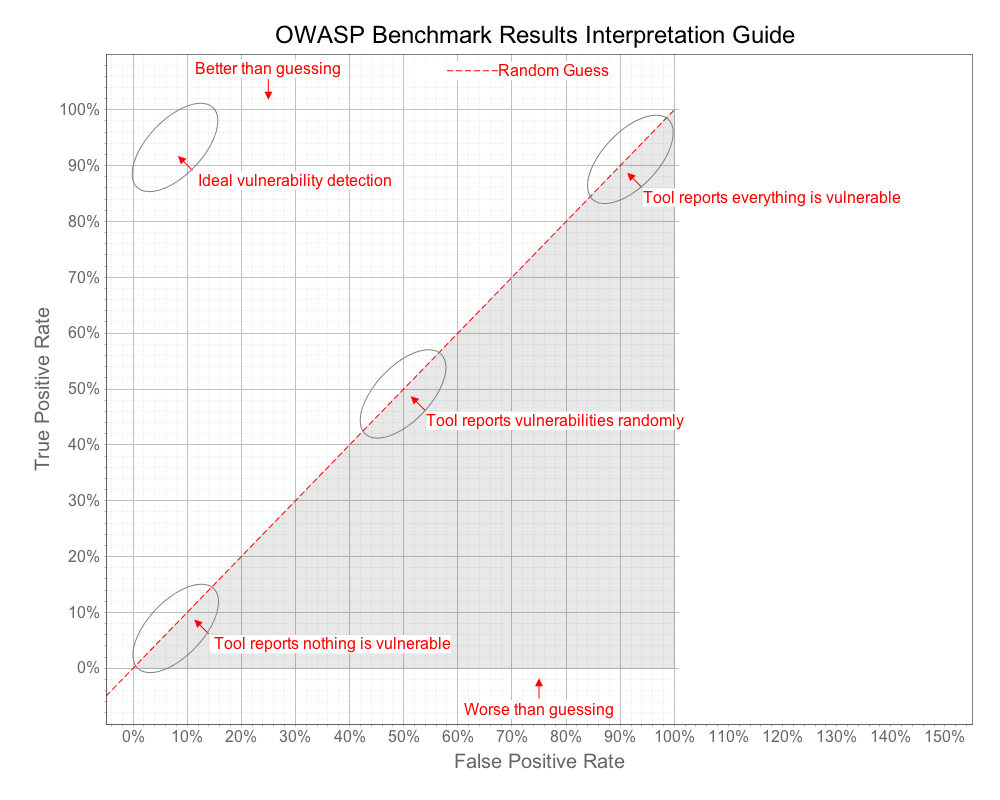
\includegraphics[width=.7\linewidth]{images/benchmark_guide.png}
%     \caption{OWASP Benchmark Scoring Guide - Youden Index interpretation \cite{owasp_benchmark_scoring}}
%     \label{fig:owasp_benchmark_scoring}
% \end{figure}

%%%% PERFORMANCE

By running KLEE and Owi on the same set of samples, some differences are visible in their outputs and in their performances (see \Cref{tab:klee_performance,tab:owi_performance}). KLEE was overall slower, with the only exception being the primes example, but was also the example that consumed less CPU but also Memory on all samples.

Unfortunately, Owi does not seem to output information regarding the travelled states, even after looking at debug logs (which depict execution instructions, but nothing was found to support a number of traversed paths).

An example of how the performance between these tools differ is with sample 3, a test where KLEE traces 306 paths. KLEE reported results consuming nearly half the CPU resources and approximately 73\% of the memory usage and 35\% of the time spent, that Owi required to run and return no results on the sample.

Sample 2 shows an even greater difference; KLEE spends nearly half the CPU and 19\% of the memory usage when compared to Owi, and does that in 1\% of the time it took Owi to analyse the same source. This scenario might be a clear indicator of Owi limitations.

% \newpage
% KLEE tests table
\begin{table}[tb]
    \begin{center}
    \caption{KLEE performance metrics}
    \begin{tabular}{c|c|c|c|c|c}
        \#$^{\mathrm{a}}$ & Success & Paths traced & CPU \textsubscript{(\%)} & Memory \textsubscript{(KB)} & Time \textsubscript{(s)}$^{\mathrm{b}}$ \\
        \hline
        \hline
        1 & YES & 3 & 99 & 98'156 & 0.29 \\
        2 & YES & 6'675 & 101 & 139'680 & 12.93 \\
        3 & YES & 305 & 93 & 99'152 & 0.72 \\
        4 & YES & 99 & 98 & 99'504 & 2.93 \\
        5 & YES & 1 & 81 & 98'036 & 0.39 \\
        6 & YES & 5 & 102 & 98'920 & 0.30 \\
        7 & YES & 5 & 87 & 97'536 & 0.37 \\
        8 & YES & 5 & 96 & 98'248 & 0.33 \\
        9 & YES & 5 & 96 & 99'236 & 0.32 \\
        \hline
        \multicolumn{6}{l}{}\\
        \multicolumn{6}{l}{$^{\mathrm{a}}$\footnotesize{Sample number}} \\
        \multicolumn{6}{l}{$^{\mathrm{b}}$\footnotesize{The best out of five runs}}
    \end{tabular}
    \end{center}
    \label{tab:klee_performance}
\end{table}

% Owi tests table
\begin{table}[tb]
    \begin{center}
    \caption{Owi performance metrics}
    \begin{tabular}{c|c|c|c|c|c}
        \#$^{\mathrm{a}}$ & Success & Paths traced & CPU \textsubscript{(\%)} & Memory \textsubscript{(KB)} & Time \textsubscript{(s)}$^{\mathrm{b}}$ \\
        \hline
        \hline
        1 & YES & \textcolor{gray}{N/A} & 108 & 110'000 & 0.05 \\
        2 & YES & \textcolor{gray}{N/A} & 200 & 725'892 & 901.51 \\
        3 & YES & \textcolor{gray}{N/A} & 199 & 134'928 & 2.10 \\
        4 & YES & \textcolor{gray}{N/A} & 204 & 145'676 & 9.90 \\
        5 & YES & \textcolor{gray}{N/A} & 205 & 151'800 & 11.13 \\
        6 & YES & \textcolor{gray}{N/A} & 116 & 120'172 & 0.06 \\
        7 & YES & \textcolor{gray}{N/A} & 115 & 119'172 & 0.06 \\
        8 & YES & \textcolor{gray}{N/A} & 118 & 118'220 & 0.05 \\
        9 & YES & \textcolor{gray}{N/A} & 123 & 121'040 & 0.05 \\
        \hline
        \multicolumn{6}{l}{}\\
        \multicolumn{6}{l}{$^{\mathrm{a}}$\footnotesize{Sample number}} \\
        \multicolumn{6}{l}{$^{\mathrm{b}}$\footnotesize{The best out of five runs}}
    \end{tabular}
    \end{center}
    \label{tab:owi_performance}
\end{table}

